%%%%%%%%%%%%%%%%%%%%%%%%%%%%%% Slide %%%%%%%%%%%%%%%%%%%%%%%%%%
\subsection{Columns}
%%%%%%%%%%%%%%%%%%%%%%%%%%%%
\begin{frame}[fragile,t]{Making Columns}
	\begin{itemize}
		\item Sometimes columns are easier for side-by-side text and figures
	\end{itemize}
\vspace{0.2in}
	\begin{columns}
		\begin{column}{0.49\textwidth}
		\begin{itemize}
			\item Example: text next to a picture
			\item See how I can use ordered lists just like I did before?
			\begin{itemize}
				\item All the same formatting rules still apply within a column
			\end{itemize}
			\item I could have also put the figure on the left and text on the right
		\end{itemize}
		\end{column}
		\begin{column}{0.49\textwidth}
		\centering
		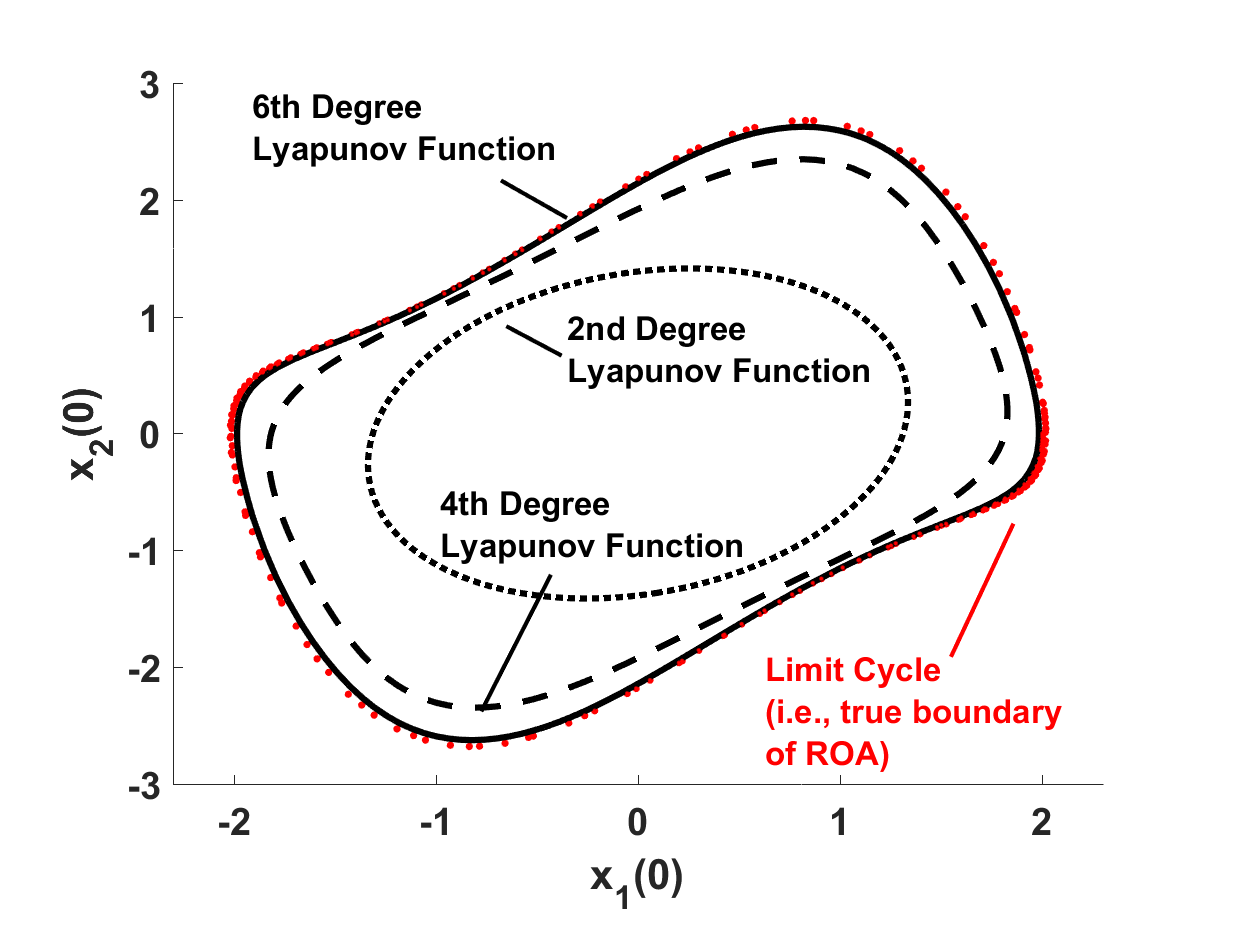
\includegraphics[width=0.9\columnwidth]{figures/my_figure.eps} 
		\end{column}
	\end{columns}
\end{frame}

%%%%%%%%%%%%%%%%%%%%%%%%%%%%
\begin{frame}[fragile,t]{Making Columns}
	\begin{itemize}
		\item Sometimes columns are easier for side-by-side text and figures
\vspace{0.2in}
		\item Or put two figures next to each other
		\begin{itemize}
			\item And add a caption
		\end{itemize}
	\end{itemize}
\vspace{0.2in}
	\begin{columns}
		\begin{column}{0.49\textwidth}
		\centering
		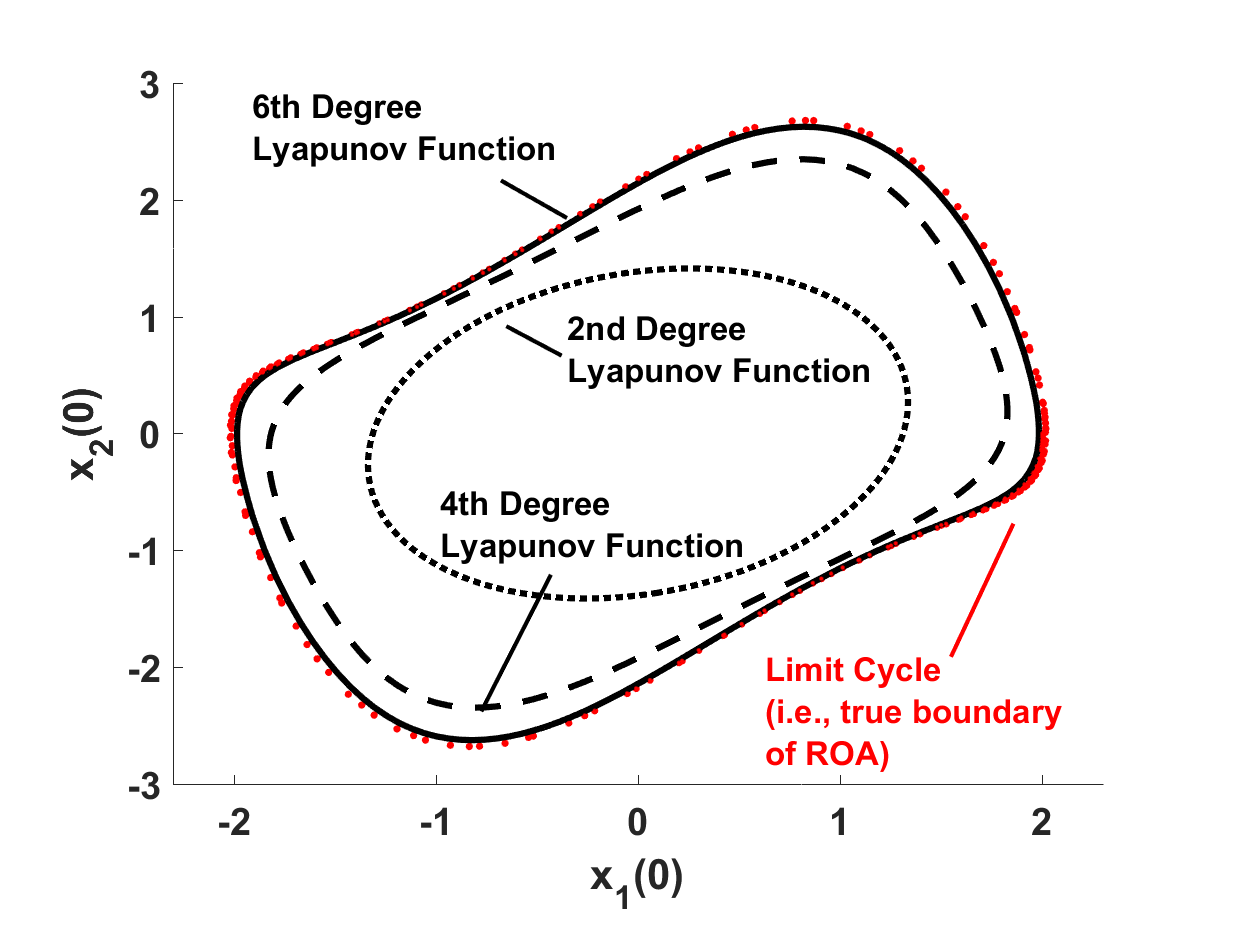
\includegraphics[width=0.9\columnwidth]{figures/my_figure.eps} 
		\\ a) caption one
		\end{column}
		\begin{column}{0.49\textwidth}
		\centering
		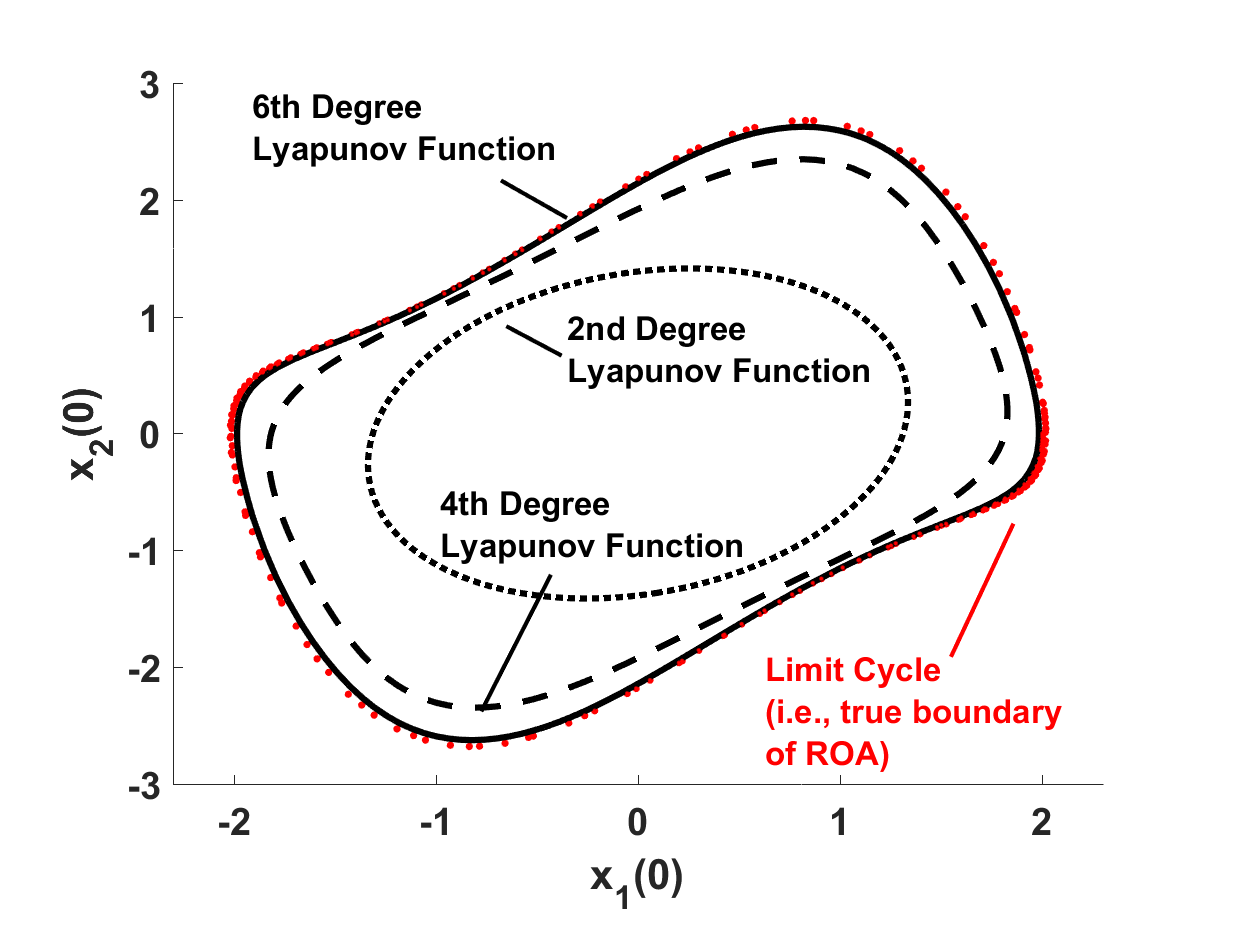
\includegraphics[width=0.9\columnwidth]{figures/my_figure.eps} 
		\\ b) caption two
		\end{column}
	\end{columns}
\end{frame}


%%%%%%%%%%%%%%%%%%%%%%%%%%%%%% Slide %%%%%%%%%%%%%%%%%%%%%%%%%%
%%%%%%%%%%%%%%%%%%%%%%%%%%%%
\begin{frame}[fragile,t]{Making Columns}
	\begin{itemize}
		\item Here's the sample code to make two columns	
{\small
	\begin{lstlisting}
\begin{columns}
	\begin{column}{0.49\textwidth}
		Add some text here
	\end{column}
	\begin{column}{0.49\textwidth}
		Add a figure here
	\end{column}
\end{columns}
	\end{lstlisting}
}
	\end{itemize}
\end{frame}

%%%%%%%%%%%%%%%%%%%%%%%%%%%%
\begin{frame}[fragile,t]{Making Columns}
	\begin{itemize}
		\item Here's the sample code to make two columns
{\small
	\begin{lstlisting}
\begin{columns}
	\begin{column}{0.49\textwidth}
		Add some text here
	\end{column}
	\begin{column}{0.49\textwidth}
		Add a figure here
	\end{column}
\end{columns}
	\end{lstlisting}
}
	\begin{itemize}
		\item Including an ordered (bulleted) list
{\small
	\begin{lstlisting}
\begin{column}{0.49\textwidth}
	\begin{itemize}
		\item Add some text here
	\end{itemize}
\end{column}
	\end{lstlisting}
}
	\end{itemize}
	\end{itemize}
\end{frame}

%%%%%%%%%%%%%%%%%%%%%%%%%%%%
\begin{frame}[fragile,t]{Making Columns}
	\begin{itemize}
		\item Here's the sample code to make two columns
{\small
	\begin{lstlisting}
\begin{columns}
	\begin{column}{0.49\textwidth}
		Add some text here
	\end{column}
	\begin{column}{0.49\textwidth}
		Add a figure here
	\end{column}
\end{columns}
	\end{lstlisting}
}
	\begin{itemize}
		\item Including a figure
{\small
	\begin{lstlisting}
\begin{column}{0.49\textwidth}
	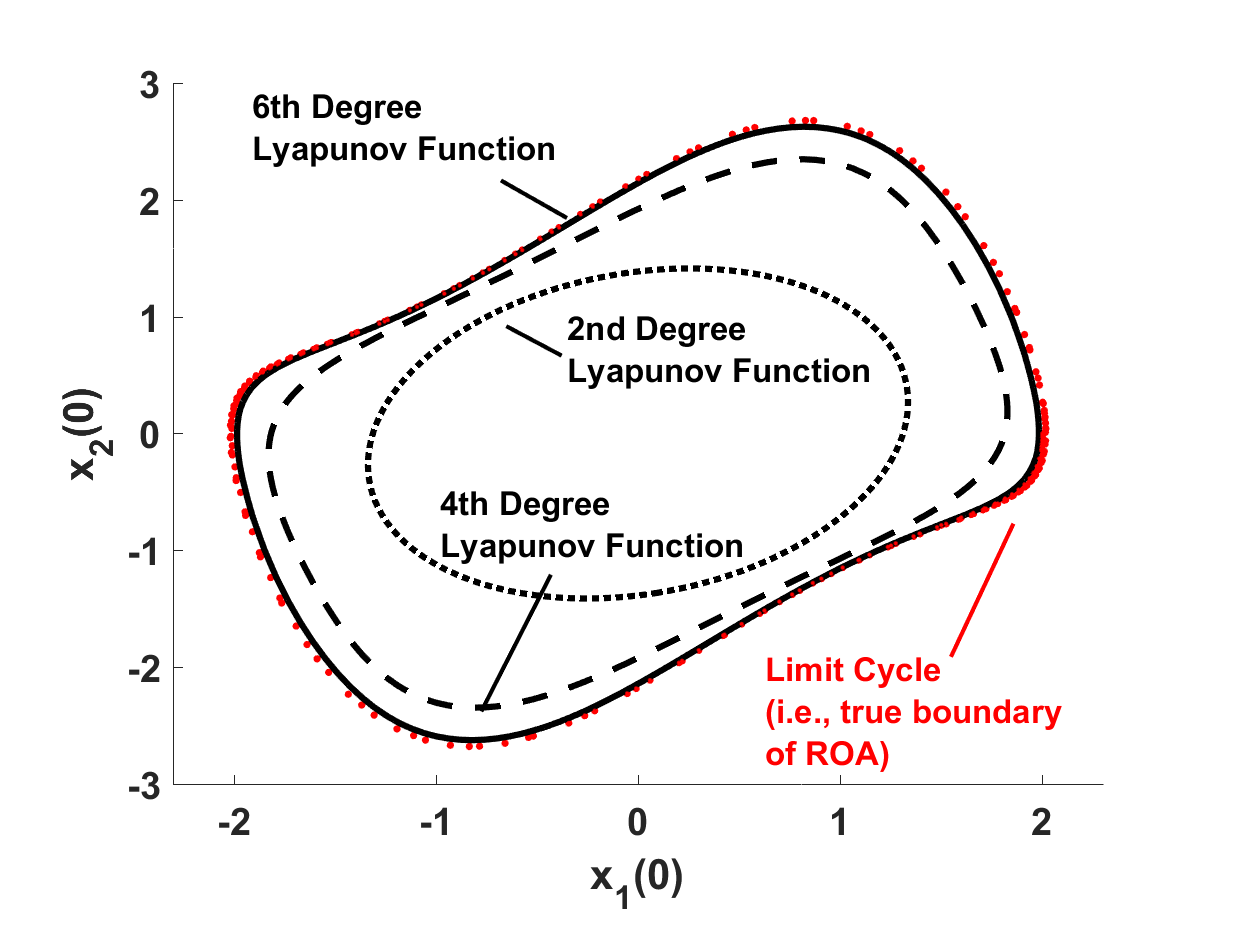
\includegraphics[width=0.9\columnwidth]{figures/my_figure.eps} 
\end{column}
	\end{lstlisting}
}
	\end{itemize}
	\end{itemize}
\end{frame}